\documentclass{article}

\usepackage{amssymb}
\usepackage{amsthm}
\usepackage{amsmath}
\usepackage{stmaryrd}
\usepackage{cancel}
\usepackage{tikz}

\usetikzlibrary{decorations.pathmorphing}

\newcommand{\es}      {\mathcal{E}}
\newcommand{\conf}[1] {\mathcal{F} \left( #1 \right) }
\newcommand{\set} [1] { \left\{ #1 \right\} }
\newcommand{\In}  [1] { \text{In} \left( #1 \right) }
\newcommand{\Min} [2] { \text{Min} \left( #1, #2 \right) }
\newcommand{\minen}   { \vdash_{min} }
\newcommand{\rc}[2]{r^{(c)}_{ #1, #2 }}
\newcommand{\rM}[2]{r^{(m)}_{ #1, #2 }}

\newcommand{\mah} [1] { { \color{red}{ Mahyar: #1 } } }

\newtheorem{thm}{Theorem}
\newtheorem{prop}[thm]{Proposition}

\theoremstyle{definition}
\newtheorem{exmp}[thm]{Example}

\theoremstyle{definition}
\newtheorem{defn}[thm]{Definition}

\begin{document}

\section{Preliminaries}

\begin{prop}\label{prop:es-induction}
For a given event structure $\es$, a set $X \in \conf{\es}$,
and an event $e$, $X \cup \set{e} \in \conf{\es}$ iff
\[ ( \forall e' \in X.\; e' \cancel{\#} e ) \wedge
  ( \exists S \subseteq X.\; S \vdash e ) \]
\end{prop}
\section{Causal Graph}

Given an event structure $\es = (E, \#, \vdash)$, we start by constructing
the lattice of \textbf{valid} configurations for $\es$. We then apply the following
transformations to this lattice:

For each edge $X \rightarrow X' = X \cup \set{e}$ in the graph,
where $X, X' \subseteq E$ and $e \in E$,
we add a new vertex $r_{X,X'}$, remove the edge $X \rightarrow X'$,
and add two new edges $X \rightarrow r_{X,X'}$, $r_{X,X'} \rightarrow X'$.

For each $S, e$ such that $S \vdash e$, we add a new vertex
(labelled as $m_{S,e}$) to the graph. For any pair of vertices
$X, X'$ in the graph, where $r_{X,X'}$ is also in the graph, we add
an edge from $m_{S,e}$ to $r_{X,X'}$ iff $S \subseteq X$ and
$\set{e} = X' \setminus X$. For consistency, we re-label the configuration vertices
such that a given vertex $X$ is re-labelled as $x_{X}$.

Informally, the $r$- and $m$-vertices are added to show the
induction steps, as defined in Prop. \ref{prop:es-induction},
for constructing the initial lattice.

\begin{exmp}\label{ex:es}
Consider the event structure $\es = (E, \#, \vdash)$,
where:
\begin{equation*}
\begin{split}
  E      & = \set{a, b, c} \\
  \#     & = \varnothing \\
  \vdash & = \set{
    (\varnothing, a), (\set{a}, b), (\set{a}, c), (\set{b}, c)
  }
\end{split}
\end{equation*}

The causal graph for $\es$ is as depicted in Fig. \ref{fig:es-causal-graph}.

\begin{figure}
\centering
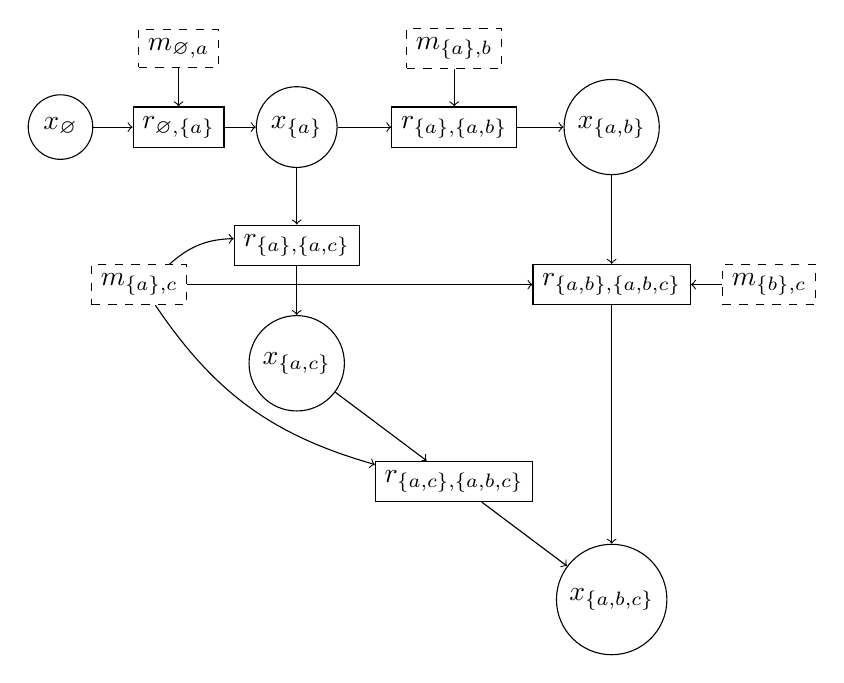
\begin{tikzpicture}
  \tikzset{
    _x/.style={circle,draw},
    r/.style={rectangle,draw},
    m/.style={rectangle,draw,dashed},
  };
  \node[_x] (_x-null) at (0,0)  {$x_{\varnothing}$};
  \node[_x] (_x-a)    at (3,0)  {$x_{\set{a}}$};
  \node[_x] (_x-ab)   at (7,0)  {$x_{\set{a,b}}$};
  \node[_x] (_x-ac)   at (3,-3) {$x_{\set{a,c}}$};
  \node[_x] (_x-abc)  at (7,-6) {$x_{\set{a,b,c}}$};

  \node[r] (r-null-a) at (1.5,0)  {$r_{\varnothing, \set{a}}$};
  \node[r] (r-a-ac)   at (3,-1.5) {$r_{\set{a}, \set{a,c}}$};
  \node[r] (r-a-ab)   at (5,0)    {$r_{\set{a}, \set{a,b}}$};
  \node[r] (r-ab-abc) at (7,-2)   {$r_{\set{a,b}, \set{a,b,c}}$};
  \node[r] (r-ac-abc) at (5,-4.5) {$r_{\set{a,c}, \set{a,b,c}}$};
  
  \node[m] (null-en-a) at (1.5, 1) {$m_{\varnothing, a}$};
  \node[m] (a-en-b)    at (5,1)    {$m_{\set{a}, b}$};
  \node[m] (a-en-c)    at (1,-2)   {$m_{\set{a}, c}$};
  \node[m] (b-en-c)    at (9,-2)   {$m_{\set{b}, c}$};

  \draw[->] (_x-null)      -- (r-null-a);
  \draw[->] (r-null-a)  -- (_x-a);
  \draw[->] (_x-a)         -- (r-a-ab);
  \draw[->] (r-a-ab)    -- (_x-ab);
  \draw[->] (_x-a)         -- (r-a-ac);
  \draw[->] (r-a-ac)    -- (_x-ac);
  \draw[->] (_x-ab)        -- (r-ab-abc);
  \draw[->] (r-ab-abc)  -- (_x-abc);
  \draw[->] (_x-ac)        -- (r-ac-abc);
  \draw[->] (r-ac-abc)  -- (_x-abc);
  \draw[->] (null-en-a) -- (r-null-a);
  \draw[->] (a-en-b)    -- (r-a-ab);
  \draw[->] (a-en-c)    -- (r-ab-abc);
  \draw[->] (b-en-c)    -- (r-ab-abc);
  \draw[->] (a-en-c) edge[bend left=20]  (r-a-ac);
  \draw[->] (a-en-c) edge[bend right=20] (r-ac-abc);
\end{tikzpicture}
\caption{Causal graph for Ex. \ref{ex:es}}
\label{fig:es-causal-graph}
\end{figure}
  

\end{exmp}

\begin{prop}
Given an event structure with $n$ events, constructing the
described causal graph requires $\mathcal{O}(2^n)$ operations.
\end{prop}
\section{Causal Model of Unsafe Behavior in Event Structure}

In this section, we define a causal model for the safety violation
in an event structure. 
More specifically, we model relations of an event structure 
with the variables and structural equations. 
We then encode the safety violation as the inclusion of a specific
subset of events in the set of configurations of the event structure.


\subsection{Causal Model of Event Structure}
Let $\mathrm{E} = (E,\#,\vdash)$ be an event structure where
$E = \s{e_1, e_2, ...,e_n}$.
Let $S \subseteq \mc{P}(E)$ be the set of unsafe behaviors.
We define the causal model
$\mc{M} = (\mc{S},\mc{F},\mc{E})$ of unsafe behavior
in $\mr{E}$ where
$\mathcal{S} = (\mathcal{U},\mathcal{V},\mathcal{R})$.
We define $\mathcal{U}$ to be empty and $\mathcal{V}$
consisting of boolean variables as follows:
\begin{align*}
    \mathcal{V} = & \s{C_{e_i,e_j} ~|~  1 \leq i < j \leq n.
    e_i \in E \wedge e_j \in E}                                \\
                  & \cup \s{EN_{s,e} ~|~ s \in \mathcal{P}(E),
    e \in E. e \not \in s }                                    \\
                  & \cup \s{M_{s,e} ~|~ s \in \mathcal{P}(E),
        e \in E. e \not \in s }
\end{align*}
Intuitively, these variables model the existence of specific elements in
each of the event structure relations: $\#$, $\vdash_{min}$, and $\vdash$.
For two events $e,e' \in E$, variables of the form $C_{e,e'}$ represent whether $e\#e'$.
Similarly, for a subset of events $s \subseteq E$ and an event $e \in E$,
we use variables of the form $M_{s,e}$ and $EN_{s,e}$ to represent
whether $s \vdash_{min} e$ and $s \vdash e$ respectively.
Finally, we use a single boolean variable, $PV$, which denote the
violation of property in the event structure.
For each variable $X \in \mathcal{V}$ we define $\vec V_X$
as a vector of all variables in $\mathcal{V} \setminus \s{X}$.
For $x,y \in \mathcal{P}(E)$ we say $x$ is covered by $y$ written $ x \prec y$ iff:
\begin{align*}
    x \subseteq y \wedge x \neq y \wedge
    (\forall z. x \subseteq z \subseteq y \Rightarrow x = z
    \vee y = z)
\end{align*}
Next we define the structural equations for each of these variables.
First, we define the structural equation of conflict variables as 
follows:
$$
    \f{C_{e,e'}} = \begin{cases}
        true  & \text{ if } e \# e' \\
        false & \text{ otherwise }
    \end{cases}
$$
We use the existing conflicts in the event structure as the initial 
value for these variables.

\noindent
For minimal enabling variables we define the following equations:
$$
    \f{M_{s,e}} = \begin{cases}
        Min(s,e) \wedge Con(s) & \text{ if } s \vdash_{min} e \\
        false                  & \text{ otherwise }
    \end{cases}
$$
Where we have:
\begin{align*}
    Con(s)   & =   \left(
    \bigwedge_{ 1\leq j<j' \leq n \wedge e_j,e_{j'} \in s}
    \neg C_{e_j,e_{j'}}
    \right)               \\
    Min(s,e) & = \left(
    \bigwedge_{s' \subseteq E. (s' \subset s \vee s \subset s')
        \wedge e \notin s'}
    \neg M_{s',e}
    \right)
\end{align*}
Intuitively, we defined the equation so that it can be affected by 
other conflict and minimal enabling variables.
For instance, assume that for some $s$ we have $s \vdash_{min} e$
thus the variable $M_{s,e}$ is true.
If we add a conflict between any pair of events in $s$ then $M_{s,e}$
becomes false.
Also if make any subset or superset of $s$ to minimally enable the $e$ then
$M_{s,e}$ becomes false.
Finally, we define the equation for the enabling variables as follows:
\begin{align*}
    \f{EN_{s,e}} & =
    \left(
    M_{s,e} \bigvee
    \left(
    \bigvee_{s'\prec s}EN_{s',e}
    \right)
    \right)
    \bigwedge
    Con(s)
\end{align*}
Intuitively, we are capturing the idea that if $s$ enables $e$ then first 
it must be consistent, and secondly either $s$ minimally enables $e$ or 
there exists a subset of $s$ that enables $e$.

\noindent Let $S \subseteq E$ be a subset of events.
We define $\varphi_S$, a boolean formula of primitive
events as follows:
\begin{align*}
    Con(S)
    \bigwedge
    \left(
        \bigwedge_{\forall e \in S}
        \left(
            \bigvee_{\forall \pi \in \pi_S} 
            \left(
                EN_{\e,\pi_1} \wedge
                EN_{\s{\pi_1},\pi_2} \wedge
                \dots
                \wedge
                EN_{\s{\pi_1,...,\pi_{n-1}},\pi_n}
            \right)
        \right)
    \right)
\end{align*}
\noindent Where $\pi_S$ is the set of all permutations of $S$.
For a permutation $\pi \in \pi_S$, where $|S| = n$, 
we write $\pi_i$ where $1 \leq i \leq n$ for the $i$th 
element of $\pi$.
Thus, for a given subset of events $S \subseteq E$, 
we can use $\varphi_S$ as the effect for which we look
for a cause.

\pagebreak


\section{HP Causality}

\subsection{Minimal Enabling as a Cause}

\begin{thm}\label{thm:hp-x-y}
Given an event structure $\es$, a cause $X = S \vdash\,e$
where $(S, e) \in \vdash$, and an effect $Y = S_f$
where $S_f \in \conf{\es}$, $X$ is a cause of $Y$
(according to the HP definition) if there is at least one path
from $m_{S,e}$ to $x_{S_f}$ in the causal graph of $\es$.
\end{thm}

\begin{proof}
We check the conditions of HP causality for the given cause and effect.

\begin{itemize}
  \item \textbf{AC1:} Both the cause and effect hold in the factual scenario;
  therefore, this condition is satisfied.
\end{itemize}

For AC2.\{a,b\}, assume $(W, w, x')$ is the witness discussed by HP.

\begin{itemize}  
  \item \textbf{AC2.a:} The idea here is to restrict the causal graph
  such that the effect holds as long as the cause.
  
  Assume the path from cause to effect is as follows:
  \begin{equation}\label{eq:validating-path}
    m_{S,e} \rightarrow
    r_{S_1,S_2} \rightarrow
    x_{S_2} \rightarrow
    r_{S_2, S_3} \rightarrow
    \cdots \rightarrow
    r_{S_{k-1}, S_k} \rightarrow x_{S_k} = x_{S_f}
  \end{equation}

  We also define $W$ as:
  \[ \left( \In{r_{S_1, S_2}} \setminus \set{x_{S_1}, m_{S,e}} \right) \cup
    \left( \bigcup_{i=2}^k \In{x_{S_i}} \setminus \set{r_{S_{i-1}, S_i}} \right) \]
   
  The elements of $W$ are shown with dotted boxes in Fig. \ref{fig:witness}.
  All variables in $W$ are set to False ($w$ is an all-False valuation).
  $x'$ sets $r_{S,e}$ to False as well.
  
  \textbf{The choice of $W$ and validating path:}
  By defining $W$ as explained above, and setting it to all-False,
  the value for each vertex of the \textit{validating} path
  (as shown in Eq. \ref{eq:validating-path})
  can be determined by its predecessor. For $i \geq 2$, we have:
  \begin{equation}\label{eq:x-Si-restrict}
    x_{S_i} = r_{S_{i-1}, S_i}
  \end{equation}
  
  By definition, each reason vertex consists of
  an \textit{enabling} and a \textit{configuration} component.
  We know the validating path is in the causal graph. Hence, for $i \geq 2$,
  the enabling component for $r_{S_i, S_{i+1}}$ is satisfied; so we have:
  \begin{equation}\label{eq:r-Si-Si+1-restrict}
    r_{S_i, S_{i+1}} = x_{S_i} \wedge \text{True} = x_{S_i}
  \end{equation}
  
  For $r_{S_1,S_2}$, after setting $W$ to all-False, we have:
  \begin{equation}\label{eq:r-S1-S2-restrict}
    r_{S_1,S_2} = \text{True} \wedge m_{S,e} = m_{S,e}
  \end{equation}
  
  \begin{figure}
\centering
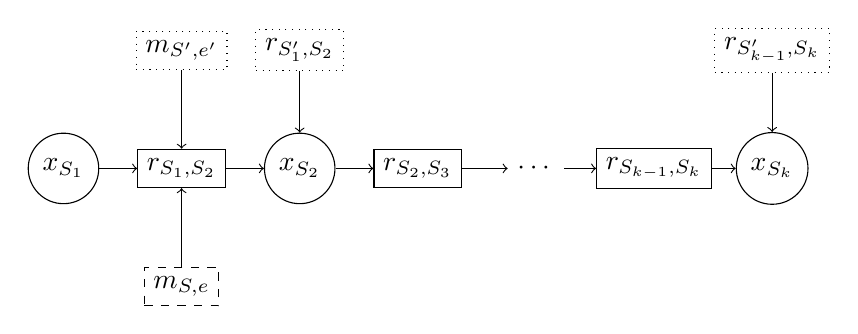
\begin{tikzpicture}
  \tikzset{
    _x/.style={circle,draw},
    r/.style={rectangle,draw},
    m/.style={rectangle,draw,dashed},
    w/.style={rectangle,draw,dotted},
  };
  \node[_x] (x-S1)       at (-1.5,0)  {$x_{S_1}$};
  \node[_x] (x-S2)       at (1.5,0)   {$x_{S_2}$};
  \node[_x] (x-Sk)       at (7.5,0)   {$x_{S_k}$};
  \node[m]  (m-S-e)      at (0,-1.5)  {$m_{S,e}$};
  \node[r]  (r-S1-S2)    at (0,0)     {$r_{S_1,S_2}$};
  \node[r]  (r-S2-S3)    at (3,0)     {$r_{S_2,S_3}$}; 
  \node[r]  (r-Sk-1-Sk)  at (6,0)     {$r_{S_{k-1},S_k}$};
  \node[w]  (m-S'-e')    at (0,1.5)   {$m_{S',e'}$};
  \node[w]  (r-S'1-S2)   at (1.5,1.5) {$r_{S'_1,S_2}$};
  \node[w]  (r-S'k-1-Sk) at (7.5,1.5) {$r_{S'_{k-1},S_k}$};
  \node     (dots)       at (4.5,0)   {$\cdots$};

  \draw[->] (x-S1)       -- (r-S1-S2);
  \draw[->] (m-S-e)      -- (r-S1-S2);
  \draw[->] (m-S'-e')    -- (r-S1-S2);
  \draw[->] (r-S1-S2)    -- (x-S2);
  \draw[->] (r-S'1-S2)   -- (x-S2);
  \draw[->] (x-S2)       -- (r-S2-S3);
  \draw[->] (r-S2-S3)    -- (dots);
  \draw[->] (dots)       -- (r-Sk-1-Sk);
  \draw[->] (r-Sk-1-Sk)  -- (x-Sk);
  \draw[->] (r-S'k-1-Sk) -- (x-Sk);
\end{tikzpicture}
\caption{Elements of $W$}
\label{fig:witness}
\end{figure}
    

  As shown in Eqs.
  \ref{eq:x-Si-restrict}, \ref{eq:r-Si-Si+1-restrict}, \ref{eq:r-S1-S2-restrict},
  Setting $m_{S,e}$ to False and $W$ to all-False will set all vertices
  in the validating path to False.

  With the witness described above, we can see that the effect $x_{S_f}$
  is also valuated as False; therefore, condition AC2.a is satisfied.
  
  
  \item \textbf{AC2.b:} After setting $m_{S,e}$ to True,
  while maintaining $W$ as all-False, $x_{S_f}$ is valuated to True again;
  this follows from the equations of the validating path when $W$ is set to all-False.
  The \textit{validating edges} for $x_{S_f}$ are shown with thick lines
  in Fig. \ref{fig:ac2.b}. Observe that, re-setting any variable $v \not\in W$
  does \textbf{not} \textit{invalidate} the specified path for $x_{S_f}$.

  \begin{figure}
\centering
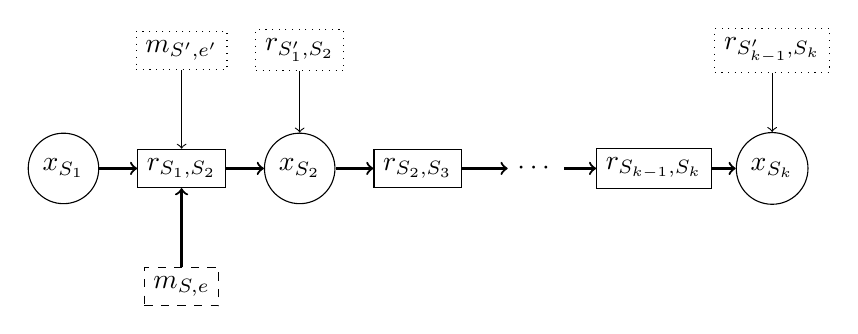
\begin{tikzpicture}
  \tikzset{
    _x/.style={circle,draw},
    r/.style={rectangle,draw},
    m/.style={rectangle,draw,dashed},
    w/.style={rectangle,draw,dotted},
  };
  \node[_x] (x-S1)       at (-1.5,0)  {$x_{S_1}$};
  \node[_x] (x-S2)       at (1.5,0)   {$x_{S_2}$};
  \node[_x] (x-Sk)       at (7.5,0)   {$x_{S_k}$};
  \node[m]  (m-S-e)      at (0,-1.5)  {$m_{S,e}$};
  \node[r]  (r-S1-S2)    at (0,0)     {$r_{S_1,S_2}$};
  \node[r]  (r-S2-S3)    at (3,0)     {$r_{S_2,S_3}$}; 
  \node[r]  (r-Sk-1-Sk)  at (6,0)     {$r_{S_{k-1},S_k}$};
  \node[w]  (m-S'-e')    at (0,1.5)   {$m_{S',e'}$};
  \node[w]  (r-S'1-S2)   at (1.5,1.5) {$r_{S'_1,S_2}$};
  \node[w]  (r-S'k-1-Sk) at (7.5,1.5) {$r_{S'_{k-1},S_k}$};
  \node     (dots)       at (4.5,0)   {$\cdots$};

  \draw[->,thick] (x-S1)       -- (r-S1-S2);
  \draw[->,thick] (m-S-e)      -- (r-S1-S2);
  \draw[->] (m-S'-e')    -- (r-S1-S2);
  \draw[->,thick] (r-S1-S2)    -- (x-S2);
  \draw[->] (r-S'1-S2)   -- (x-S2);
  \draw[->,thick] (x-S2)       -- (r-S2-S3);
  \draw[->,thick] (r-S2-S3)    -- (dots);
  \draw[->,thick] (dots)       -- (r-Sk-1-Sk);
  \draw[->,thick] (r-Sk-1-Sk)  -- (x-Sk);
  \draw[->] (r-S'k-1-Sk) -- (x-Sk);
\end{tikzpicture}
\caption{\textit{Validating} path for $X_{S_f}$}
\label{fig:ac2.b}
\end{figure}
    

  \item \textbf{AC3:} As our cause is a singleton,
  this condition is also satisfied.
\end{itemize}

\end{proof}

\begin{thm}\label{thm:hp-x-disj-Y}
Given an event structure $\es$, a cause $X = S \vdash\,e$
where $(S, e) \in \vdash$, and an effect $Y = \bigvee_{f} S_{f}$
where $\forall f.\;S_f \in \conf{\es}$, $X$ is a cause of $Y$
(according to the HP definition) if there exists $f$ such that
there is at least one path from $m_{S,e}$ to $x_{S_f}$
in the causal graph of $\es$.
\end{thm}

\begin{proof}
Assume there is a path from $m_{S,e}$ to $x_{S_f}$ for some $f$.
Also assume $W$ is defined as in Thm. \ref{thm:hp-x-y}. For this problem,
we construct the new witness $W'$ as follows:
\[ W' = W \cup \left( \bigcup_{f' \neq f} x_{S_{f'}} \right) \]

$W'$ is set to all-False, as before.

With the new witness, both AC2.a and AC2.b can be satisfied
for the new problem.
\end{proof}

\begin{thm}\label{thm:hp-x-conj-Y}
Given an event structure $\es$, a cause $X = S \vdash\,e$
where $(S, e) \in \vdash$, and an effect $Y = \bigwedge_{f} S_{f}$
where $\forall f.\;S_f \in \conf{\es}$, $X$ is a cause of $Y$
(according to the HP definition) if there exists $f$ such that
there is at least one path from $m_{S,e}$ to $x_{S_f}$
in the causal graph of $\es$.  
\end{thm}

\begin{proof}
The set $W$ is selected just as done in Thm. \ref{thm:hp-x-disj-Y}.
For any $w \in W \cap Y$, we set $w$ to True.
\end{proof}

\begin{thm}\label{thm:hp-X-Y}
Given an event structure $\es$,
a cause $X = \set{S_1 \vdash\, e_1, \cdots, S_k \vdash\, e_k}$
where $(S_i, e_i) \in \vdash$, and an effect $Y = x_{S_f}$
where $S_f \in \conf{\es}$, $X$ is not a cause of $Y$. 
\end{thm}

\begin{proof}
The result holds if there is no path from $X$ to $Y$.
Assume there is a path from $X$ to $Y$.
this path starts from a vertex $m_{S_i,e_i}$, where $(S_i \vdash e_i) \in X$.
As stated in Thm. \ref{thm:hp-x-y}, $S_i \vdash e_i$ is a cause of $Y$.
Hence, AC3 does not hold for $X$.
\end{proof}

\subsection{False Minimal Enabling as a Cause}

In the previous section, we showed how to check causality for
true minimal enabling relations
(i.e. $S \vdash e =$ True in the given event structure).
Now we want to improve the existing causal graph
to include false minimal enabling relations as well.

Given event structure $\es = (E, \#, \vdash)$,
For each $S \subseteq E$ and $e \in E$, we define vertex $r_{S,e}$.
The value associated with this vertex will be as follows:

\[ m_{S,e} =
  \begin{cases}
    \Min{S}{e}   & \text{if } S \vdash_{min} e \\
    \text{False} & \text{otherwise}
  \end{cases}
\]

Where $\Min{S}{e}$ is defined as follows:
\[ \Min{S}{e} =
  \bigwedge_{S' \subseteq E.\;(S' \subset S) \vee (S \subset S')}
  \neg m_{S',e}
\]

Informally, if $S$ minimally enables $e$, no pure sub- or super-set of $S$
minimally enables $e$. 
\newcommand{\ra}    { \rightarrow }
\newcommand{\sem}[1]{ \llbracket #1 \rrbracket }

\begin{exmp}
\begin{figure}
\centering
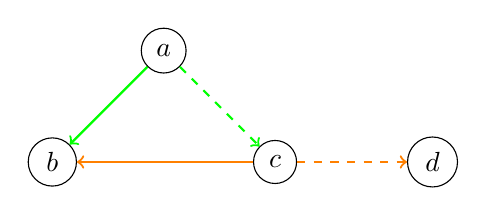
\begin{tikzpicture} [
    node distance={20mm},
    main/.style = {draw, circle},
    s/.style = {->,thick},
    d/.style = {->,thick,dashed}
  ]
  \node[main] (b) {$b$};
  \node[main] (a) [above right of=b] {$a$};
  \node[main] (c) [below right of=a] {$c$};
  \node[main] (d) [right of=c] {$d$};
  \draw[thick,green,->] (a) -- (b);
  \draw[thick,green,->,dashed] (a) -- (c);
  \draw[thick,orange,->] (c) -- (b);
  \draw[thick,orange,->,dashed] (c) -- (d);
\end{tikzpicture}
\caption{Failure of blacklist property}
\label{fig:blacklist}
\end{figure}

Blacklisted nodes are nodes in the network that must not
be reachable.
Let's assume the network in Fig. \ref{fig:blacklist} as
an example where the node $d$ is blacklisted.
For simplicity we assume that we require
$d$ not reachable only from $a$.
Consider the following DyNetKAT program for this network:
\begin{equation*}
\begin{aligned}[c]
    P   & = p!1                             \\
    Q   & = q!1                             \\
    N   & = F \oplus p?1;N_p \oplus q?1;N_q \\
    N_p & = F_p \oplus q?1;F_{pq}           \\
    N_q & = F_q \oplus p?1;F_{pq}           \\
    F   & = a\ra b \oplus c\ra b            \\
\end{aligned}
\qquad\qquad
\begin{aligned}[c]
    F_p         & = a\ra c \oplus c\ra b \oplus a\ra b \\
    F_q         & = a\ra b \oplus c\ra d               \\
    F_{pq}      & = a\ra c \oplus c\ra d \oplus a\ra d \\
    SDN         & = \delta_{\mathcal{L}} (N
    \parallel P \parallel Q)                           \\
    \mathcal{L} & = \set{p!1,p?1,q?1,q?1}                \\
\end{aligned}
\end{equation*}
We assume that there are two concurrent processes for updating
the switches $a$ and $c$.
Let we use $p$ and $q$ to denote $rcfg(p,1)$ and
$rcfg(q,1)$ respectively.
Thus, $p$ and $q$ replace the solid green and orange
paths in the network with dashed paths respectively.

Obviously, executing both $rcfg_{p,1}$ and $rcfg_{q,1}$ leads
to a state where we can forward the $\sigma_a$ to $d$.
To find the cause of error, let $\es = \sem{SDN}$ and $M$
be the causal model of $\es$, where we encode the unsafe behavior 
as:
\begin{equation*}
  \varphi = \exists X \in \conf{\es}.\;\exists e \in X.\;l(e) = a \ra d
\end{equation*}

The property above sets the value of $\varphi$ to True if $\es$ 
contains a configuration with an event labeled $a \ra d$.
In $SDN$ there are two orders of execution for $p$ and $q$; hence,
there are two events for each of these labels in $\es$ 
and thus, there are two events with the label $a \ra d$ as well.
So, let's consider events $p_1,p_2$ with label $p$,
events $q_1,q_2$ with label $q$ and events $ad_1,ad_2$ 
with label $a \ra d$ in $E$. Fig. \ref{fig:blacklist:lattice}
shows a portion of the $\conf{\es}$ lattice, which consists of configurations
which lead to events labeled with $a\ra d$.

\newcommand{\crd}[4][above]{
  \node[draw,circle,inner sep=2pt,fill,label={[#1]:#4}] at (#2,#3) {};
}

\begin{figure}
\centering
\begin{tikzpicture}
  \crd{0}{0}{$\emptyset$}
  \crd[left]{-2}{1}{$\set{p_1}$}
  \crd[left]{-2}{2}{$\set{p_1,q_1}$}
  \crd[left]{-2}{3}{$\set{p_1,q_1,ad_1}$}
  \crd[right]{2}{1}{$\set{q_2}$}
  \crd[right]{2}{2}{$\set{p_2,q_2}$}
  \crd[right]{2}{3}{$\set{p_2,q_2,ad_2}$}
  \draw [ultra thick] (-2,1) -- (-2,2);
  \draw [ultra thick] (-2,2) -- (-2,3);
  \draw [ultra thick] (0,0) -- (2,1);
  \draw [ultra thick] (0,0) -- (-2,1);
  \draw [ultra thick] (2,1) -- (2,2);
  \draw [ultra thick] (2,1) -- (2,3);
\end{tikzpicture}
\caption{Configurations lattice for the blacklist network}
\label{fig:blacklist:lattice}
\end{figure}


\usetikzlibrary{shapes.geometric}


\begin{figure}
\centering
\begin{tikzpicture}
  \tikzset{
    _x/.style={ellipse,draw},
    r/.style={rectangle,draw,font=\tiny},
    m/.style={rectangle,draw,dashed,font=\tiny},
    c/.style={rectangle,draw,dotted,font=\tiny},
  }

  \node[_x] (x-null)    at (0,0)  {$x_{\varnothing}$};
  \node[_x] (x-p1)      at (-2.5,4) {$x_{ \set{p_1} }$};
  \node[_x] (x-p1q1)    at (-2.5,8) {$x_{ \set{p_1,q_1} }$};
  \node[_x] (x-p1q1ad1) at (-2.5,12) {$x_{ \set{p_1,q_1,ad_1} }$};
  \node[_x] (x-q2)      at (2.5,4)  {$x_{ \set{q_2} }$};
  \node[_x] (x-q2p2)    at (2.5,8)  {$x_{ \set{q_2,p_2} }$};
  \node[_x] (x-q2p2ad2) at (2.5,12)  {$x_{ \set{q_2,p_2,ad_2} }$};

  \node[r] (rc-null-p1)      at (-2.5,1.25) {$\rc{\varnothing}{ \set{p_1} }$};
  \node[r] (rm-null-p1)      at (-2.5,2.5) {$\rM{\varnothing}{ \set{p_1} }$};
  \node[r] (rc-p1-p1q1)      at (-2.5,5.25) {$\rc{ \set{p_1} }{ \set{p_1,q_1} }$};
  \node[r] (rm-p1-p1q1)      at (-2.5,6.5) {$\rM{ \set{p_1} }{ \set{p_1,q_1} }$};
  \node[r] (rc-p1q1-p1q1ad1) at (-2.5,9.25) {$\rc{ \set{p_1,q_1} }{ \set{p_1,q_1,ad_1} }$};
  \node[r] (rm-p1q1-p1q1ad1) at (-2.5,10.5) {$\rM{ \set{p_1,q_1} }{ \set{p_1,q_1,ad_1} }$};

  \node[r] (rc-null-q2)      at (2.5,1.25) {$\rc{\varnothing}{ \set{q_2} }$};
  \node[r] (rm-null-q2)      at (2.5,2.5) {$\rM{\varnothing}{ \set{q_2} }$};
  \node[r] (rc-q2-q2p2)      at (2.5,5.25) {$\rc{ \set{q_2} }{ \set{q_2,p_2} }$};
  \node[r] (rm-q2-q2p2)      at (2.5,6.5) {$\rM{ \set{q_2} }{ \set{q_2,p_2} }$};
  \node[r] (rc-q2p2-q2p2ad2) at (2.5,9.25) {$\rc{ \set{q_2,p_2} }{ \set{q_2,p_2,ad_2} }$};
  \node[r] (rm-q2p2-q2p2ad2) at (2.5,10.5) {$\rM{ \set{q_2,p_2} }{ \set{q_2,p_2,ad_2} }$};

  \node[m] (m-null-p1)       at (-5,2.5)  {$m_{\varnothing, p_1 }$};
  \node[m] (m-p1-q1)         at (-5,6.5)  {$m_{\set{p_1}, q_1 }$};
  \node[m] (m-q1-ad1)        at (-5,10.5) {$m_{\set{q_1}, ad_1 }$};

  \node[m] (m-null-q2)       at (5,2.5)  {$m_{\varnothing, p_1 }$};
  \node[m] (m-q2-p2)         at (5,6.5)  {$m_{\set{q_2}, p_2 }$};
  \node[m] (m-p2-ad2)        at (5,10.5) {$m_{\set{p_2}, ad_2 }$};

  \node[c] (c-p1-q1)         at (-5,5.25) {$c_{ p_1,q_1 }$};
  \node[c] (c-p1-ad1)        at (-5,8)    {$c_{ p_1,ad_1 }$};
  \node[c] (c-q1-ad1)        at (-5,9.25) {$c_{ q_1,ad_1 }$};

  \node[c] (c-q2-p2)         at (5,5.25) {$c_{ q_2,p_2 }$};
  \node[c] (c-q2-ad2)        at (5,8)    {$c_{ q_2,ad_2 }$};
  \node[c] (c-p2-ad2)        at (5,9.25) {$c_{ q_1,ad_2 }$};

  \draw[->] (x-null)          -- (rc-null-p1);
  \draw[->] (rc-null-p1)      -- (rm-null-p1);
  \draw[->] (rm-null-p1)      -- (x-p1);
  \draw[->] (x-p1)            -- (rc-p1-p1q1);
  \draw[->] (rc-p1-p1q1)      -- (rm-p1-p1q1);
  \draw[->] (rm-p1-p1q1)      -- (x-p1q1);
  \draw[->] (x-p1q1)          -- (rc-p1q1-p1q1ad1);
  \draw[->] (rc-p1q1-p1q1ad1) -- (rm-p1q1-p1q1ad1);
  \draw[->] (rm-p1q1-p1q1ad1) -- (x-p1q1ad1);
  
  \draw[->] (x-null)          -- (rc-null-q2);
  \draw[->] (rc-null-q2)      -- (rm-null-q2);
  \draw[->] (rm-null-q2)      -- (x-q2);
  \draw[->] (x-q2)            -- (rc-q2-q2p2);
  \draw[->] (rc-q2-q2p2)      -- (rm-q2-q2p2);
  \draw[->] (rm-q2-q2p2)      -- (x-q2p2);
  \draw[->] (x-q2p2)          -- (rc-q2p2-q2p2ad2);
  \draw[->] (rc-q2p2-q2p2ad2) -- (rm-q2p2-q2p2ad2);
  \draw[->] (rm-q2p2-q2p2ad2) -- (x-q2p2ad2);

  \draw[->] (m-null-p1)       -- (rm-null-p1);
  \draw[->] (m-p1-q1)         -- (rm-p1-p1q1);
  \draw[->] (m-q1-ad1)        -- (rm-p1q1-p1q1ad1);

  \draw[->] (m-null-q2)       -- (rm-null-q2);
  \draw[->] (m-q2-p2)         -- (rm-q2-q2p2);
  \draw[->] (m-p2-ad2)        -- (rm-q2p2-q2p2ad2);

  \draw[->] (c-p1-q1)         -- (rc-p1-p1q1);
  \draw[->] (c-p1-ad1)        -- (rc-p1q1-p1q1ad1);
  \draw[->] (c-q1-ad1)        -- (rc-p1q1-p1q1ad1);

  \draw[->] (c-q2-p2)         -- (rc-q2-q2p2);
  \draw[->] (c-q2-ad2)        -- (rc-q2p2-q2p2ad2);
  \draw[->] (c-p2-ad2)        -- (rc-q2p2-q2p2ad2);
\end{tikzpicture}
\caption{Causal graph for the blacklist network}
\label{fig:blacklist:causal-graph}
\end{figure}


The causal graph for this event structure is presented in Fig. \ref{fig:blacklist:causal-graph}.
We claim that $p_1 \cancel{\#} q_1$ is a cause of $\varphi$. To check, we only need to see
if there is a path from $c_{p_1,q_1}$ to either $x_{p_1,q_1,ad_1}$ or $x_{q_2,p_2,ad_2}$.
In this case, there is such a path; so the causality claim holds.
$q_2 \cancel{\#} p_2$ is also a cause of $\varphi$, due to symmetry.
\end{exmp}

\end{document}